% Options for packages loaded elsewhere
\PassOptionsToPackage{unicode}{hyperref}
\PassOptionsToPackage{hyphens}{url}
%
\documentclass[
]{article}
\usepackage{amsmath,amssymb}
\usepackage{iftex}
\ifPDFTeX
  \usepackage[T1]{fontenc}
  \usepackage[utf8]{inputenc}
  \usepackage{textcomp} % provide euro and other symbols
\else % if luatex or xetex
  \usepackage{unicode-math} % this also loads fontspec
  \defaultfontfeatures{Scale=MatchLowercase}
  \defaultfontfeatures[\rmfamily]{Ligatures=TeX,Scale=1}
\fi
\usepackage{lmodern}
\ifPDFTeX\else
  % xetex/luatex font selection
\fi
% Use upquote if available, for straight quotes in verbatim environments
\IfFileExists{upquote.sty}{\usepackage{upquote}}{}
\IfFileExists{microtype.sty}{% use microtype if available
  \usepackage[]{microtype}
  \UseMicrotypeSet[protrusion]{basicmath} % disable protrusion for tt fonts
}{}
\makeatletter
\@ifundefined{KOMAClassName}{% if non-KOMA class
  \IfFileExists{parskip.sty}{%
    \usepackage{parskip}
  }{% else
    \setlength{\parindent}{0pt}
    \setlength{\parskip}{6pt plus 2pt minus 1pt}}
}{% if KOMA class
  \KOMAoptions{parskip=half}}
\makeatother
\usepackage{xcolor}
\usepackage[margin=1in]{geometry}
\usepackage{color}
\usepackage{fancyvrb}
\newcommand{\VerbBar}{|}
\newcommand{\VERB}{\Verb[commandchars=\\\{\}]}
\DefineVerbatimEnvironment{Highlighting}{Verbatim}{commandchars=\\\{\}}
% Add ',fontsize=\small' for more characters per line
\usepackage{framed}
\definecolor{shadecolor}{RGB}{248,248,248}
\newenvironment{Shaded}{\begin{snugshade}}{\end{snugshade}}
\newcommand{\AlertTok}[1]{\textcolor[rgb]{0.94,0.16,0.16}{#1}}
\newcommand{\AnnotationTok}[1]{\textcolor[rgb]{0.56,0.35,0.01}{\textbf{\textit{#1}}}}
\newcommand{\AttributeTok}[1]{\textcolor[rgb]{0.13,0.29,0.53}{#1}}
\newcommand{\BaseNTok}[1]{\textcolor[rgb]{0.00,0.00,0.81}{#1}}
\newcommand{\BuiltInTok}[1]{#1}
\newcommand{\CharTok}[1]{\textcolor[rgb]{0.31,0.60,0.02}{#1}}
\newcommand{\CommentTok}[1]{\textcolor[rgb]{0.56,0.35,0.01}{\textit{#1}}}
\newcommand{\CommentVarTok}[1]{\textcolor[rgb]{0.56,0.35,0.01}{\textbf{\textit{#1}}}}
\newcommand{\ConstantTok}[1]{\textcolor[rgb]{0.56,0.35,0.01}{#1}}
\newcommand{\ControlFlowTok}[1]{\textcolor[rgb]{0.13,0.29,0.53}{\textbf{#1}}}
\newcommand{\DataTypeTok}[1]{\textcolor[rgb]{0.13,0.29,0.53}{#1}}
\newcommand{\DecValTok}[1]{\textcolor[rgb]{0.00,0.00,0.81}{#1}}
\newcommand{\DocumentationTok}[1]{\textcolor[rgb]{0.56,0.35,0.01}{\textbf{\textit{#1}}}}
\newcommand{\ErrorTok}[1]{\textcolor[rgb]{0.64,0.00,0.00}{\textbf{#1}}}
\newcommand{\ExtensionTok}[1]{#1}
\newcommand{\FloatTok}[1]{\textcolor[rgb]{0.00,0.00,0.81}{#1}}
\newcommand{\FunctionTok}[1]{\textcolor[rgb]{0.13,0.29,0.53}{\textbf{#1}}}
\newcommand{\ImportTok}[1]{#1}
\newcommand{\InformationTok}[1]{\textcolor[rgb]{0.56,0.35,0.01}{\textbf{\textit{#1}}}}
\newcommand{\KeywordTok}[1]{\textcolor[rgb]{0.13,0.29,0.53}{\textbf{#1}}}
\newcommand{\NormalTok}[1]{#1}
\newcommand{\OperatorTok}[1]{\textcolor[rgb]{0.81,0.36,0.00}{\textbf{#1}}}
\newcommand{\OtherTok}[1]{\textcolor[rgb]{0.56,0.35,0.01}{#1}}
\newcommand{\PreprocessorTok}[1]{\textcolor[rgb]{0.56,0.35,0.01}{\textit{#1}}}
\newcommand{\RegionMarkerTok}[1]{#1}
\newcommand{\SpecialCharTok}[1]{\textcolor[rgb]{0.81,0.36,0.00}{\textbf{#1}}}
\newcommand{\SpecialStringTok}[1]{\textcolor[rgb]{0.31,0.60,0.02}{#1}}
\newcommand{\StringTok}[1]{\textcolor[rgb]{0.31,0.60,0.02}{#1}}
\newcommand{\VariableTok}[1]{\textcolor[rgb]{0.00,0.00,0.00}{#1}}
\newcommand{\VerbatimStringTok}[1]{\textcolor[rgb]{0.31,0.60,0.02}{#1}}
\newcommand{\WarningTok}[1]{\textcolor[rgb]{0.56,0.35,0.01}{\textbf{\textit{#1}}}}
\usepackage{graphicx}
\makeatletter
\def\maxwidth{\ifdim\Gin@nat@width>\linewidth\linewidth\else\Gin@nat@width\fi}
\def\maxheight{\ifdim\Gin@nat@height>\textheight\textheight\else\Gin@nat@height\fi}
\makeatother
% Scale images if necessary, so that they will not overflow the page
% margins by default, and it is still possible to overwrite the defaults
% using explicit options in \includegraphics[width, height, ...]{}
\setkeys{Gin}{width=\maxwidth,height=\maxheight,keepaspectratio}
% Set default figure placement to htbp
\makeatletter
\def\fps@figure{htbp}
\makeatother
\setlength{\emergencystretch}{3em} % prevent overfull lines
\providecommand{\tightlist}{%
  \setlength{\itemsep}{0pt}\setlength{\parskip}{0pt}}
\setcounter{secnumdepth}{-\maxdimen} % remove section numbering
\ifLuaTeX
  \usepackage{selnolig}  % disable illegal ligatures
\fi
\IfFileExists{bookmark.sty}{\usepackage{bookmark}}{\usepackage{hyperref}}
\IfFileExists{xurl.sty}{\usepackage{xurl}}{} % add URL line breaks if available
\urlstyle{same}
\hypersetup{
  pdfauthor={Abhijith R Upadhya},
  hidelinks,
  pdfcreator={LaTeX via pandoc}}

\author{Abhijith R Upadhya}
\date{2025-08-24}

\begin{document}

\hypertarget{violence-on-women---analysis-and-prediction}{%
\section{\texorpdfstring{\textbf{Violence on Women - Analysis and
Prediction}}{Violence on Women - Analysis and Prediction}}\label{violence-on-women---analysis-and-prediction}}

\begin{figure}
\centering
\includegraphics[width=\textwidth,height=5.20833in]{https://media.licdn.com/dms/image/v2/D5612AQEZkTV5_SqH_Q/article-cover_image-shrink_720_1280/article-cover_image-shrink_720_1280/0/1714268684747?e=1735776000\&v=beta\&t=LJQxBUAlioMMrau9BuLC-MnOJp_WCXc24ly0H0NFh3E}
\caption{Source: Media Licdn.}
\end{figure}

\hypertarget{introduction}{%
\subsection{Introduction}\label{introduction}}

In this analysis, we explore a dataset on domestic violence and examine
several variables to understand their distribution, relationships, and
potential predictive power for violence occurrence. Key variables
include Age, Income, Education, Employment, and Marital Status. The aim
is to preprocess the data, visualize patterns, and implement machine
learning models to predict occurrences of violence.

\hypertarget{libraries}{%
\subsection{Libraries}\label{libraries}}

\begin{Shaded}
\begin{Highlighting}[]
\FunctionTok{library}\NormalTok{(e1071)}
\FunctionTok{library}\NormalTok{(rpart)}
\FunctionTok{library}\NormalTok{(randomForest)}
\FunctionTok{library}\NormalTok{(class)}
\FunctionTok{library}\NormalTok{(ROSE)}
\FunctionTok{library}\NormalTok{(caret)}
\FunctionTok{library}\NormalTok{(gridExtra)}
\FunctionTok{library}\NormalTok{(tidyr)}
\FunctionTok{library}\NormalTok{(RColorBrewer)}
\FunctionTok{library}\NormalTok{(tidyverse)}
\FunctionTok{library}\NormalTok{(corrplot)}
\FunctionTok{library}\NormalTok{(ggplot2)}
\FunctionTok{library}\NormalTok{(viridis)}
\FunctionTok{library}\NormalTok{(dplyr)}
\end{Highlighting}
\end{Shaded}

\hypertarget{loading-the-dataset}{%
\subsection{Loading the dataset}\label{loading-the-dataset}}

\begin{Shaded}
\begin{Highlighting}[]
\CommentTok{\# Read the dataset}
\NormalTok{df }\OtherTok{\textless{}{-}} \FunctionTok{read.csv}\NormalTok{(}\StringTok{"Domestic\_violence.csv"}\NormalTok{)}
\end{Highlighting}
\end{Shaded}

\hypertarget{data-transformation}{%
\subsection{Data Transformation}\label{data-transformation}}

\hypertarget{data-preparation-and-cleaning}{%
\subsubsection{Data Preparation and
Cleaning}\label{data-preparation-and-cleaning}}

Loading Packages and Dataset: Load necessary libraries for data
manipulation, visualization, and modeling. The dataset is read and
cleaned to prepare for analysis. Handling Missing Values and Duplicate
Records: Check for and handle null values, duplicates, and inconsistent
entries.

Feature Engineering: Binarize categorical variables like
Marital\_status, Education, Employment, and Violence for better model
compatibility. Additionally, some columns are trimmed and converted to
binary form where applicable.

\begin{Shaded}
\begin{Highlighting}[]
\CommentTok{\# Data preparation}
\NormalTok{df }\OtherTok{\textless{}{-}}\NormalTok{ df }\SpecialCharTok{\%\textgreater{}\%} 
  \FunctionTok{select}\NormalTok{(}\SpecialCharTok{{-}}\StringTok{\textquotesingle{}Sl.No.\textquotesingle{}}\NormalTok{) }\SpecialCharTok{\%\textgreater{}\%}
  \FunctionTok{mutate}\NormalTok{(}\FunctionTok{across}\NormalTok{(}\FunctionTok{c}\NormalTok{(}\StringTok{\textquotesingle{}Education\textquotesingle{}}\NormalTok{, }\StringTok{\textquotesingle{}Employment\textquotesingle{}}\NormalTok{, }\StringTok{\textquotesingle{}Marital\_status\textquotesingle{}}\NormalTok{), as.character)) }\SpecialCharTok{\%\textgreater{}\%}
  \FunctionTok{mutate}\NormalTok{(}\AttributeTok{Employment =} \FunctionTok{trimws}\NormalTok{(Employment))}

\CommentTok{\# Check dimensions}
\FunctionTok{dim}\NormalTok{(df)}
\end{Highlighting}
\end{Shaded}

\begin{verbatim}
## [1] 347   6
\end{verbatim}

\begin{Shaded}
\begin{Highlighting}[]
\CommentTok{\# Check data types}
\FunctionTok{str}\NormalTok{(df)}
\end{Highlighting}
\end{Shaded}

\begin{verbatim}
## 'data.frame':    347 obs. of  6 variables:
##  $ Age           : int  30 47 24 22 50 21 30 27 20 18 ...
##  $ Education     : chr  "secondary" "tertiary" "tertiary" "tertiary" ...
##  $ Employment    : chr  "unemployed" "unemployed" "unemployed" "unemployed" ...
##  $ Income        : int  0 0 0 0 0 0 0 0 0 0 ...
##  $ Marital_status: chr  "married" "married" "unmarred" "unmarred" ...
##  $ Violence      : chr  "yes" "no" "no" "no" ...
\end{verbatim}

\begin{Shaded}
\begin{Highlighting}[]
\CommentTok{\# Check for null values}
\FunctionTok{colSums}\NormalTok{(}\FunctionTok{is.na}\NormalTok{(df))}
\end{Highlighting}
\end{Shaded}

\begin{verbatim}
##            Age      Education     Employment         Income Marital_status 
##              0              0              0              0              0 
##       Violence 
##              0
\end{verbatim}

\begin{Shaded}
\begin{Highlighting}[]
\CommentTok{\# Count distinct values for each column}
\FunctionTok{sapply}\NormalTok{(df, }\ControlFlowTok{function}\NormalTok{(x) }\FunctionTok{length}\NormalTok{(}\FunctionTok{unique}\NormalTok{(x)))}
\end{Highlighting}
\end{Shaded}

\begin{verbatim}
##            Age      Education     Employment         Income Marital_status 
##             39              4              3             29              2 
##       Violence 
##              2
\end{verbatim}

\begin{Shaded}
\begin{Highlighting}[]
\CommentTok{\# Binarize the dataset}
\NormalTok{df }\OtherTok{\textless{}{-}}\NormalTok{ df }\SpecialCharTok{\%\textgreater{}\%}
  \FunctionTok{mutate}\NormalTok{(}
    \AttributeTok{marital\_binary =} \FunctionTok{case\_when}\NormalTok{(}
\NormalTok{      Marital\_status }\SpecialCharTok{==} \StringTok{\textquotesingle{}married\textquotesingle{}} \SpecialCharTok{\textasciitilde{}} \DecValTok{1}\NormalTok{,}
\NormalTok{      Marital\_status }\SpecialCharTok{==} \StringTok{\textquotesingle{}unmarred\textquotesingle{}} \SpecialCharTok{\textasciitilde{}} \DecValTok{0}
\NormalTok{    ),}
    \AttributeTok{Violence =} \FunctionTok{case\_when}\NormalTok{(}
\NormalTok{      Violence }\SpecialCharTok{==} \StringTok{\textquotesingle{}yes\textquotesingle{}} \SpecialCharTok{\textasciitilde{}} \DecValTok{1}\NormalTok{,}
\NormalTok{      Violence }\SpecialCharTok{==} \StringTok{\textquotesingle{}no\textquotesingle{}} \SpecialCharTok{\textasciitilde{}} \DecValTok{0}
\NormalTok{    ),}
    \AttributeTok{education\_binary =} \FunctionTok{case\_when}\NormalTok{(}
\NormalTok{      Education }\SpecialCharTok{==} \StringTok{\textquotesingle{}none\textquotesingle{}} \SpecialCharTok{\textasciitilde{}} \DecValTok{0}\NormalTok{,}
\NormalTok{      Education }\SpecialCharTok{==} \StringTok{\textquotesingle{}primary\textquotesingle{}} \SpecialCharTok{\textasciitilde{}} \DecValTok{1}\NormalTok{,}
\NormalTok{      Education }\SpecialCharTok{==} \StringTok{\textquotesingle{}secondary\textquotesingle{}} \SpecialCharTok{\textasciitilde{}} \DecValTok{2}\NormalTok{,}
\NormalTok{      Education }\SpecialCharTok{==} \StringTok{\textquotesingle{}tertiary\textquotesingle{}} \SpecialCharTok{\textasciitilde{}} \DecValTok{3}
\NormalTok{    ),}
    \AttributeTok{employment\_binary =} \FunctionTok{case\_when}\NormalTok{(}
\NormalTok{      Employment }\SpecialCharTok{==} \StringTok{\textquotesingle{}unemployed\textquotesingle{}} \SpecialCharTok{\textasciitilde{}} \DecValTok{0}\NormalTok{,}
\NormalTok{      Employment }\SpecialCharTok{==} \StringTok{\textquotesingle{}semi employed\textquotesingle{}} \SpecialCharTok{\textasciitilde{}} \DecValTok{1}\NormalTok{,}
\NormalTok{      Employment }\SpecialCharTok{==} \StringTok{\textquotesingle{}employed\textquotesingle{}} \SpecialCharTok{\textasciitilde{}} \DecValTok{2}
\NormalTok{    )}
\NormalTok{  )}

\CommentTok{\# Check zero income count}
\FunctionTok{sum}\NormalTok{(df}\SpecialCharTok{$}\NormalTok{Income }\SpecialCharTok{==} \DecValTok{0}\NormalTok{)}
\end{Highlighting}
\end{Shaded}

\begin{verbatim}
## [1] 272
\end{verbatim}

\begin{Shaded}
\begin{Highlighting}[]
\CommentTok{\# Check outliers {-} Employed/Semi{-}employed with zero income}
\NormalTok{mask }\OtherTok{\textless{}{-}}\NormalTok{ df }\SpecialCharTok{\%\textgreater{}\%}
  \FunctionTok{filter}\NormalTok{(Income }\SpecialCharTok{==} \DecValTok{0} \SpecialCharTok{\&}\NormalTok{ (Employment }\SpecialCharTok{==} \StringTok{"employed"} \SpecialCharTok{|}\NormalTok{ Employment }\SpecialCharTok{==} \StringTok{"semi employed"}\NormalTok{))}
\FunctionTok{print}\NormalTok{(mask)}
\end{Highlighting}
\end{Shaded}

\begin{verbatim}
## [1] Age               Education         Employment        Income           
## [5] Marital_status    Violence          marital_binary    education_binary 
## [9] employment_binary
## <0 rows> (or 0-length row.names)
\end{verbatim}

\begin{Shaded}
\begin{Highlighting}[]
\CommentTok{\# Check duplicates}
\NormalTok{duplicate\_rows }\OtherTok{\textless{}{-}}\NormalTok{ df[}\FunctionTok{duplicated}\NormalTok{(df), ]}
\FunctionTok{cat}\NormalTok{(}\StringTok{"Number of duplicate rows:"}\NormalTok{, }\FunctionTok{nrow}\NormalTok{(duplicate\_rows))}
\end{Highlighting}
\end{Shaded}

\begin{verbatim}
## Number of duplicate rows: 133
\end{verbatim}

\begin{Shaded}
\begin{Highlighting}[]
\CommentTok{\# Summary statistics}
\FunctionTok{summary}\NormalTok{(df)}
\end{Highlighting}
\end{Shaded}

\begin{verbatim}
##       Age         Education          Employment            Income     
##  Min.   :15.00   Length:347         Length:347         Min.   :    0  
##  1st Qu.:23.00   Class :character   Class :character   1st Qu.:    0  
##  Median :30.00   Mode  :character   Mode  :character   Median :    0  
##  Mean   :31.38                                         Mean   : 2111  
##  3rd Qu.:39.50                                         3rd Qu.:    0  
##  Max.   :60.00                                         Max.   :35000  
##  Marital_status        Violence      marital_binary   education_binary
##  Length:347         Min.   :0.0000   Min.   :0.0000   Min.   :0.000   
##  Class :character   1st Qu.:0.0000   1st Qu.:1.0000   1st Qu.:1.000   
##  Mode  :character   Median :0.0000   Median :1.0000   Median :1.000   
##                     Mean   :0.2478   Mean   :0.8646   Mean   :1.461   
##                     3rd Qu.:0.0000   3rd Qu.:1.0000   3rd Qu.:2.000   
##                     Max.   :1.0000   Max.   :1.0000   Max.   :3.000   
##  employment_binary
##  Min.   :0.0000   
##  1st Qu.:0.0000   
##  Median :0.0000   
##  Mean   :0.2853   
##  3rd Qu.:0.0000   
##  Max.   :2.0000
\end{verbatim}

\hypertarget{data-visualisation-and-analysis}{%
\subsection{Data Visualisation and
Analysis}\label{data-visualisation-and-analysis}}

\hypertarget{histograms-and-density-plots}{%
\subsubsection{1. Histograms and Density
Plots:}\label{histograms-and-density-plots}}

Age Distribution: Examines the age distribution within the dataset.

\begin{Shaded}
\begin{Highlighting}[]
\CommentTok{\# Create histograms}
\FunctionTok{par}\NormalTok{(}\AttributeTok{mfrow =} \FunctionTok{c}\NormalTok{(}\DecValTok{1}\NormalTok{, }\DecValTok{2}\NormalTok{))}
\NormalTok{hist\_age }\OtherTok{\textless{}{-}} \FunctionTok{ggplot}\NormalTok{(df, }\FunctionTok{aes}\NormalTok{(}\AttributeTok{x =}\NormalTok{ Age)) }\SpecialCharTok{+}
  \FunctionTok{geom\_histogram}\NormalTok{(}\FunctionTok{aes}\NormalTok{(}\AttributeTok{y =} \FunctionTok{after\_stat}\NormalTok{(density)), }\AttributeTok{bins =} \DecValTok{30}\NormalTok{) }\SpecialCharTok{+}
  \FunctionTok{geom\_density}\NormalTok{() }\SpecialCharTok{+}
  \FunctionTok{theme\_minimal}\NormalTok{() }\SpecialCharTok{+}
  \FunctionTok{labs}\NormalTok{(}\AttributeTok{title =} \StringTok{"Age Distribution"}\NormalTok{)}
\end{Highlighting}
\end{Shaded}

Income Distribution: Analyzes the income distribution with a focus on
zero-income cases.

\begin{Shaded}
\begin{Highlighting}[]
\NormalTok{hist\_income }\OtherTok{\textless{}{-}} \FunctionTok{ggplot}\NormalTok{(df, }\FunctionTok{aes}\NormalTok{(}\AttributeTok{x =}\NormalTok{ Income)) }\SpecialCharTok{+}
  \FunctionTok{geom\_histogram}\NormalTok{(}\AttributeTok{bins =} \DecValTok{30}\NormalTok{) }\SpecialCharTok{+}
  \FunctionTok{theme\_minimal}\NormalTok{() }\SpecialCharTok{+}
  \FunctionTok{labs}\NormalTok{(}\AttributeTok{title =} \StringTok{"Income Distribution"}\NormalTok{)}

\FunctionTok{grid.arrange}\NormalTok{(hist\_age, hist\_income, }\AttributeTok{ncol =} \DecValTok{2}\NormalTok{)}
\end{Highlighting}
\end{Shaded}

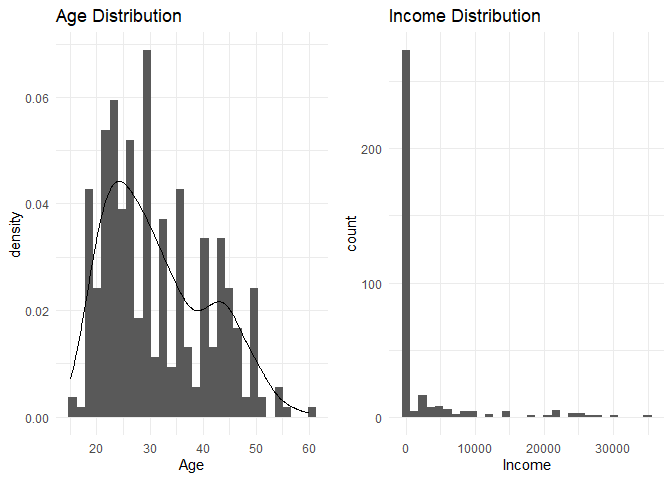
\includegraphics{Violence-On-Women_files/figure-latex/income_distribution-1.pdf}

\hypertarget{boxplot-of-income}{%
\subsubsection{2. Boxplot of Income:}\label{boxplot-of-income}}

A boxplot reveals the spread and presence of any potential outliers
within the income data.

\begin{Shaded}
\begin{Highlighting}[]
\CommentTok{\# Create boxplot}
\FunctionTok{ggplot}\NormalTok{(df, }\FunctionTok{aes}\NormalTok{(}\AttributeTok{y =}\NormalTok{ Income)) }\SpecialCharTok{+}
  \FunctionTok{geom\_boxplot}\NormalTok{(}\AttributeTok{width =} \FloatTok{0.2}\NormalTok{) }\SpecialCharTok{+}
  \FunctionTok{theme\_minimal}\NormalTok{() }\SpecialCharTok{+}
  \FunctionTok{labs}\NormalTok{(}\AttributeTok{title =} \StringTok{"Income Distribution Boxplot"}\NormalTok{)}
\end{Highlighting}
\end{Shaded}

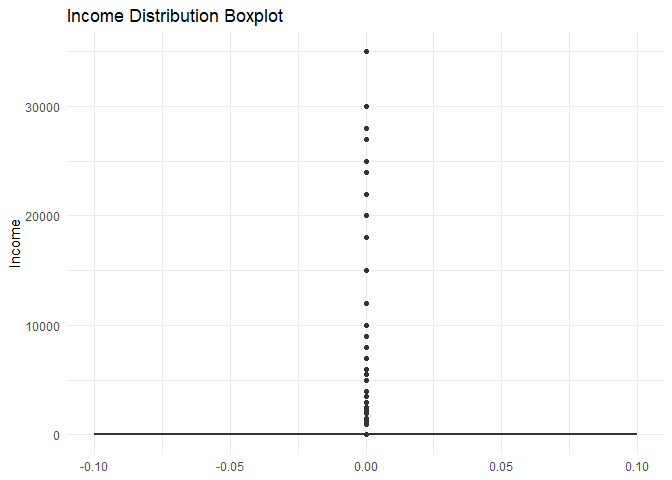
\includegraphics{Violence-On-Women_files/figure-latex/income_boxplot-1.pdf}

\hypertarget{correlation-between-features}{%
\subsubsection{3. Correlation Between
Features}\label{correlation-between-features}}

A correlation matrix visualizes relationships among features. Insights
from this plot help guide the selection of features for machine learning
models.

\begin{Shaded}
\begin{Highlighting}[]
\CommentTok{\# Correlation matrix}
\NormalTok{df\_binary }\OtherTok{\textless{}{-}}\NormalTok{ df }\SpecialCharTok{\%\textgreater{}\%}
  \FunctionTok{select}\NormalTok{(Age, education\_binary, employment\_binary, Income, marital\_binary, Violence)}

\NormalTok{correlation\_matrix }\OtherTok{\textless{}{-}} \FunctionTok{cor}\NormalTok{(df\_binary)}
\FunctionTok{corrplot}\NormalTok{(correlation\_matrix, }
         \AttributeTok{method =} \StringTok{"color"}\NormalTok{, }
         \AttributeTok{type =} \StringTok{"upper"}\NormalTok{, }
         \AttributeTok{addCoef.col =} \StringTok{"black"}\NormalTok{,}
         \AttributeTok{number.cex =} \FloatTok{0.7}\NormalTok{,}
         \AttributeTok{col =} \FunctionTok{viridis}\NormalTok{(}\DecValTok{100}\NormalTok{))}
\end{Highlighting}
\end{Shaded}

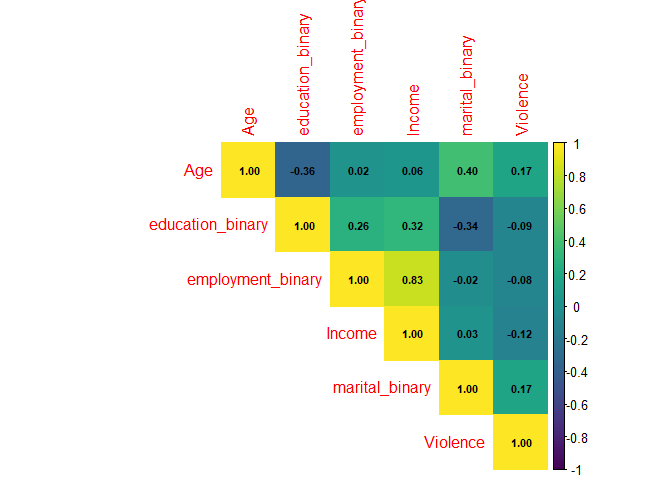
\includegraphics{Violence-On-Women_files/figure-latex/correlation_matrix-1.pdf}

\begin{Shaded}
\begin{Highlighting}[]
\CommentTok{\# Define color palettes}
\NormalTok{palette }\OtherTok{\textless{}{-}} \FunctionTok{c}\NormalTok{(}\StringTok{"\#0096c7"}\NormalTok{, }\StringTok{"\#00b4d8"}\NormalTok{, }\StringTok{"\#48cae4"}\NormalTok{, }\StringTok{"\#90e0ef"}\NormalTok{)}
\NormalTok{palette\_pie }\OtherTok{\textless{}{-}} \FunctionTok{c}\NormalTok{(}\StringTok{"\#0096c7"}\NormalTok{, }\StringTok{"\#e3f2fd"}\NormalTok{, }\StringTok{"\#bbdefb"}\NormalTok{, }\StringTok{"\#90caf9"}\NormalTok{)}
\end{Highlighting}
\end{Shaded}

\hypertarget{relevant-pie-charts}{%
\subsubsection{4. Relevant Pie Charts:}\label{relevant-pie-charts}}

Violence Distribution: Displays the percentage distribution of reported
domestic violence cases.

Marital Status, Employment, and Education: These charts provide a visual
overview of the dataset's composition in terms of marital status,
employment, and education levels.

\begin{Shaded}
\begin{Highlighting}[]
\CommentTok{\# Display first 10 rows}
\FunctionTok{head}\NormalTok{(df, }\DecValTok{10}\NormalTok{)}
\end{Highlighting}
\end{Shaded}

\begin{verbatim}
##    Age Education Employment Income Marital_status Violence marital_binary
## 1   30 secondary unemployed      0        married        1              1
## 2   47  tertiary unemployed      0        married        0              1
## 3   24  tertiary unemployed      0       unmarred        0              0
## 4   22  tertiary unemployed      0       unmarred        0              0
## 5   50   primary unemployed      0        married        1              1
## 6   21  tertiary unemployed      0       unmarred        1              0
## 7   30  tertiary unemployed      0        married        0              1
## 8   27  tertiary unemployed      0        married        0              1
## 9   20  tertiary unemployed      0       unmarred        0              0
## 10  18 secondary unemployed      0        married        0              1
##    education_binary employment_binary
## 1                 2                 0
## 2                 3                 0
## 3                 3                 0
## 4                 3                 0
## 5                 1                 0
## 6                 3                 0
## 7                 3                 0
## 8                 3                 0
## 9                 3                 0
## 10                2                 0
\end{verbatim}

\begin{Shaded}
\begin{Highlighting}[]
\CommentTok{\# Distribution of features {-} Create 4 pie charts}
\CommentTok{\# Violence View}
\NormalTok{p1 }\OtherTok{\textless{}{-}}\NormalTok{ df }\SpecialCharTok{\%\textgreater{}\%}
  \FunctionTok{count}\NormalTok{(Violence) }\SpecialCharTok{\%\textgreater{}\%}
  \FunctionTok{mutate}\NormalTok{(}
    \AttributeTok{prop =}\NormalTok{ n}\SpecialCharTok{/}\FunctionTok{sum}\NormalTok{(n),}
    \AttributeTok{label =} \FunctionTok{c}\NormalTok{(}\StringTok{"No"}\NormalTok{, }\StringTok{"Yes"}\NormalTok{),}
    \AttributeTok{pct =} \FunctionTok{paste0}\NormalTok{(}\FunctionTok{round}\NormalTok{(prop }\SpecialCharTok{*} \DecValTok{100}\NormalTok{, }\DecValTok{1}\NormalTok{), }\StringTok{"\%"}\NormalTok{)}
\NormalTok{  ) }\SpecialCharTok{\%\textgreater{}\%}
  \FunctionTok{ggplot}\NormalTok{(}\FunctionTok{aes}\NormalTok{(}\AttributeTok{x =} \StringTok{""}\NormalTok{, }\AttributeTok{y =}\NormalTok{ prop, }\AttributeTok{fill =} \FunctionTok{factor}\NormalTok{(label))) }\SpecialCharTok{+}
  \FunctionTok{geom\_bar}\NormalTok{(}\AttributeTok{stat =} \StringTok{"identity"}\NormalTok{, }\AttributeTok{width =} \DecValTok{1}\NormalTok{) }\SpecialCharTok{+}
  \FunctionTok{coord\_polar}\NormalTok{(}\StringTok{"y"}\NormalTok{, }\AttributeTok{start =} \DecValTok{0}\NormalTok{) }\SpecialCharTok{+}
  \FunctionTok{geom\_text}\NormalTok{(}\FunctionTok{aes}\NormalTok{(}\AttributeTok{label =}\NormalTok{ pct), }\AttributeTok{position =} \FunctionTok{position\_stack}\NormalTok{(}\AttributeTok{vjust =} \FloatTok{0.5}\NormalTok{)) }\SpecialCharTok{+}
  \FunctionTok{scale\_fill\_manual}\NormalTok{(}\AttributeTok{values =}\NormalTok{ palette\_pie) }\SpecialCharTok{+}
  \FunctionTok{labs}\NormalTok{(}\AttributeTok{title =} \StringTok{"Violence View"}\NormalTok{) }\SpecialCharTok{+}
  \FunctionTok{theme\_void}\NormalTok{() }\SpecialCharTok{+}
  \FunctionTok{theme}\NormalTok{(}\AttributeTok{legend.title =} \FunctionTok{element\_blank}\NormalTok{())}

\CommentTok{\# Marital View}
\NormalTok{p2 }\OtherTok{\textless{}{-}}\NormalTok{ df }\SpecialCharTok{\%\textgreater{}\%}
  \FunctionTok{count}\NormalTok{(Marital\_status) }\SpecialCharTok{\%\textgreater{}\%}
  \FunctionTok{mutate}\NormalTok{(}
    \AttributeTok{prop =}\NormalTok{ n}\SpecialCharTok{/}\FunctionTok{sum}\NormalTok{(n),}
    \AttributeTok{pct =} \FunctionTok{paste0}\NormalTok{(}\FunctionTok{round}\NormalTok{(prop }\SpecialCharTok{*} \DecValTok{100}\NormalTok{, }\DecValTok{1}\NormalTok{), }\StringTok{"\%"}\NormalTok{)}
\NormalTok{  ) }\SpecialCharTok{\%\textgreater{}\%}
  \FunctionTok{ggplot}\NormalTok{(}\FunctionTok{aes}\NormalTok{(}\AttributeTok{x =} \StringTok{""}\NormalTok{, }\AttributeTok{y =}\NormalTok{ prop, }\AttributeTok{fill =}\NormalTok{ Marital\_status)) }\SpecialCharTok{+}
  \FunctionTok{geom\_bar}\NormalTok{(}\AttributeTok{stat =} \StringTok{"identity"}\NormalTok{, }\AttributeTok{width =} \DecValTok{1}\NormalTok{) }\SpecialCharTok{+}
  \FunctionTok{coord\_polar}\NormalTok{(}\StringTok{"y"}\NormalTok{, }\AttributeTok{start =} \DecValTok{0}\NormalTok{) }\SpecialCharTok{+}
  \FunctionTok{geom\_text}\NormalTok{(}\FunctionTok{aes}\NormalTok{(}\AttributeTok{label =}\NormalTok{ pct), }\AttributeTok{position =} \FunctionTok{position\_stack}\NormalTok{(}\AttributeTok{vjust =} \FloatTok{0.5}\NormalTok{)) }\SpecialCharTok{+}
  \FunctionTok{scale\_fill\_manual}\NormalTok{(}\AttributeTok{values =}\NormalTok{ palette\_pie) }\SpecialCharTok{+}
  \FunctionTok{labs}\NormalTok{(}\AttributeTok{title =} \StringTok{"Marital View"}\NormalTok{) }\SpecialCharTok{+}
  \FunctionTok{theme\_void}\NormalTok{() }\SpecialCharTok{+}
  \FunctionTok{theme}\NormalTok{(}\AttributeTok{legend.title =} \FunctionTok{element\_blank}\NormalTok{())}

\CommentTok{\# Employment View}
\NormalTok{p3 }\OtherTok{\textless{}{-}}\NormalTok{ df }\SpecialCharTok{\%\textgreater{}\%}
  \FunctionTok{count}\NormalTok{(Employment) }\SpecialCharTok{\%\textgreater{}\%}
  \FunctionTok{mutate}\NormalTok{(}
    \AttributeTok{prop =}\NormalTok{ n}\SpecialCharTok{/}\FunctionTok{sum}\NormalTok{(n),}
    \AttributeTok{pct =} \FunctionTok{paste0}\NormalTok{(}\FunctionTok{round}\NormalTok{(prop }\SpecialCharTok{*} \DecValTok{100}\NormalTok{, }\DecValTok{1}\NormalTok{), }\StringTok{"\%"}\NormalTok{)}
\NormalTok{  ) }\SpecialCharTok{\%\textgreater{}\%}
  \FunctionTok{ggplot}\NormalTok{(}\FunctionTok{aes}\NormalTok{(}\AttributeTok{x =} \StringTok{""}\NormalTok{, }\AttributeTok{y =}\NormalTok{ prop, }\AttributeTok{fill =}\NormalTok{ Employment)) }\SpecialCharTok{+}
  \FunctionTok{geom\_bar}\NormalTok{(}\AttributeTok{stat =} \StringTok{"identity"}\NormalTok{, }\AttributeTok{width =} \DecValTok{1}\NormalTok{) }\SpecialCharTok{+}
  \FunctionTok{coord\_polar}\NormalTok{(}\StringTok{"y"}\NormalTok{, }\AttributeTok{start =} \DecValTok{0}\NormalTok{) }\SpecialCharTok{+}
  \FunctionTok{geom\_text}\NormalTok{(}\FunctionTok{aes}\NormalTok{(}\AttributeTok{label =}\NormalTok{ pct), }\AttributeTok{position =} \FunctionTok{position\_stack}\NormalTok{(}\AttributeTok{vjust =} \FloatTok{0.5}\NormalTok{)) }\SpecialCharTok{+}
  \FunctionTok{scale\_fill\_manual}\NormalTok{(}\AttributeTok{values =}\NormalTok{ palette\_pie) }\SpecialCharTok{+}
  \FunctionTok{labs}\NormalTok{(}\AttributeTok{title =} \StringTok{"Employment View"}\NormalTok{) }\SpecialCharTok{+}
  \FunctionTok{theme\_void}\NormalTok{() }\SpecialCharTok{+}
  \FunctionTok{theme}\NormalTok{(}\AttributeTok{legend.title =} \FunctionTok{element\_blank}\NormalTok{())}

\CommentTok{\# Education View}
\NormalTok{p4 }\OtherTok{\textless{}{-}}\NormalTok{ df }\SpecialCharTok{\%\textgreater{}\%}
  \FunctionTok{count}\NormalTok{(Education) }\SpecialCharTok{\%\textgreater{}\%}
  \FunctionTok{mutate}\NormalTok{(}
    \AttributeTok{prop =}\NormalTok{ n}\SpecialCharTok{/}\FunctionTok{sum}\NormalTok{(n),}
    \AttributeTok{pct =} \FunctionTok{paste0}\NormalTok{(}\FunctionTok{round}\NormalTok{(prop }\SpecialCharTok{*} \DecValTok{100}\NormalTok{, }\DecValTok{1}\NormalTok{), }\StringTok{"\%"}\NormalTok{)}
\NormalTok{  ) }\SpecialCharTok{\%\textgreater{}\%}
  \FunctionTok{ggplot}\NormalTok{(}\FunctionTok{aes}\NormalTok{(}\AttributeTok{x =} \StringTok{""}\NormalTok{, }\AttributeTok{y =}\NormalTok{ prop, }\AttributeTok{fill =}\NormalTok{ Education)) }\SpecialCharTok{+}
  \FunctionTok{geom\_bar}\NormalTok{(}\AttributeTok{stat =} \StringTok{"identity"}\NormalTok{, }\AttributeTok{width =} \DecValTok{1}\NormalTok{) }\SpecialCharTok{+}
  \FunctionTok{coord\_polar}\NormalTok{(}\StringTok{"y"}\NormalTok{, }\AttributeTok{start =} \DecValTok{0}\NormalTok{) }\SpecialCharTok{+}
  \FunctionTok{geom\_text}\NormalTok{(}\FunctionTok{aes}\NormalTok{(}\AttributeTok{label =}\NormalTok{ pct), }\AttributeTok{position =} \FunctionTok{position\_stack}\NormalTok{(}\AttributeTok{vjust =} \FloatTok{0.5}\NormalTok{)) }\SpecialCharTok{+}
  \FunctionTok{scale\_fill\_manual}\NormalTok{(}\AttributeTok{values =}\NormalTok{ palette\_pie) }\SpecialCharTok{+}
  \FunctionTok{labs}\NormalTok{(}\AttributeTok{title =} \StringTok{"Education View"}\NormalTok{) }\SpecialCharTok{+}
  \FunctionTok{theme\_void}\NormalTok{() }\SpecialCharTok{+}
  \FunctionTok{theme}\NormalTok{(}\AttributeTok{legend.title =} \FunctionTok{element\_blank}\NormalTok{())}

\CommentTok{\# Arrange all pie charts in a grid}
\FunctionTok{grid.arrange}\NormalTok{(p1, p2, p3, p4, }\AttributeTok{ncol =} \DecValTok{2}\NormalTok{)}
\end{Highlighting}
\end{Shaded}

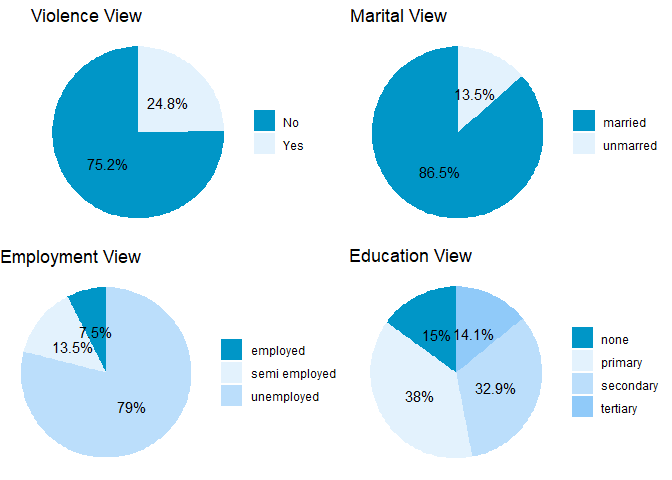
\includegraphics{Violence-On-Women_files/figure-latex/thefour_piecharts-1.pdf}

\hypertarget{scatter-plots-of-age-and-income-for-violence-cases-highlight-potential-patterns.}{%
\subsubsection{Scatter plots of Age and Income for violence cases
highlight potential
patterns.}\label{scatter-plots-of-age-and-income-for-violence-cases-highlight-potential-patterns.}}

\begin{Shaded}
\begin{Highlighting}[]
\CommentTok{\# Age \& Income x Violence}
\NormalTok{violence\_data }\OtherTok{\textless{}{-}}\NormalTok{ df }\SpecialCharTok{\%\textgreater{}\%} \FunctionTok{filter}\NormalTok{(Violence }\SpecialCharTok{==} \DecValTok{1}\NormalTok{)}

\CommentTok{\# Create scatter plots for Age and Income}
\NormalTok{p5 }\OtherTok{\textless{}{-}} \FunctionTok{ggplot}\NormalTok{(violence\_data, }\FunctionTok{aes}\NormalTok{(}\AttributeTok{x =}\NormalTok{ Age, }\AttributeTok{y =}\NormalTok{ Age)) }\SpecialCharTok{+}
  \FunctionTok{geom\_point}\NormalTok{() }\SpecialCharTok{+}
  \FunctionTok{theme\_minimal}\NormalTok{()}

\NormalTok{p6 }\OtherTok{\textless{}{-}} \FunctionTok{ggplot}\NormalTok{(violence\_data, }\FunctionTok{aes}\NormalTok{(}\AttributeTok{x =}\NormalTok{ Income, }\AttributeTok{y =}\NormalTok{ Age)) }\SpecialCharTok{+}
  \FunctionTok{geom\_point}\NormalTok{() }\SpecialCharTok{+}
  \FunctionTok{theme\_minimal}\NormalTok{()}

\FunctionTok{grid.arrange}\NormalTok{(p5, p6, }\AttributeTok{ncol =} \DecValTok{2}\NormalTok{)}
\end{Highlighting}
\end{Shaded}

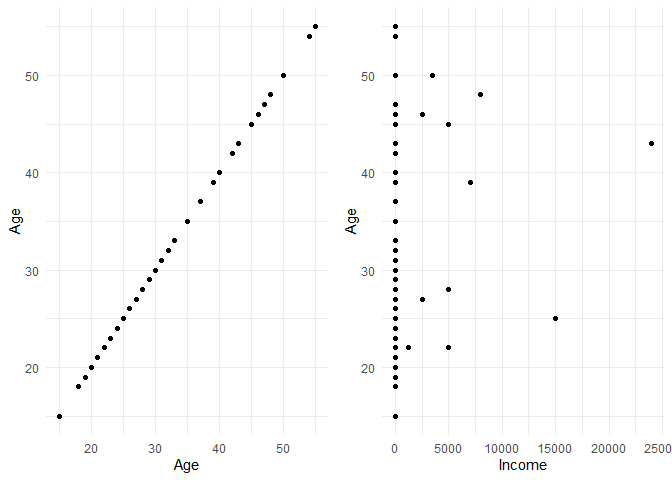
\includegraphics{Violence-On-Women_files/figure-latex/ageincome_scatterplot-1.pdf}

\hypertarget{education-and-violence-bar-plot-demonstrates-the-relationship-between-education-levels-and-violence-incidence.}{%
\subsubsection{Education and Violence Bar Plot: Demonstrates the
relationship between education levels and violence
incidence.}\label{education-and-violence-bar-plot-demonstrates-the-relationship-between-education-levels-and-violence-incidence.}}

\begin{Shaded}
\begin{Highlighting}[]
\CommentTok{\# Education x Violence}
\FunctionTok{ggplot}\NormalTok{(df, }\FunctionTok{aes}\NormalTok{(}\AttributeTok{y =}\NormalTok{ Education, }\AttributeTok{fill =} \FunctionTok{factor}\NormalTok{(Violence))) }\SpecialCharTok{+}
  \FunctionTok{geom\_bar}\NormalTok{(}\AttributeTok{position =} \StringTok{"dodge"}\NormalTok{) }\SpecialCharTok{+}
  \FunctionTok{scale\_fill\_manual}\NormalTok{(}\AttributeTok{values =}\NormalTok{ palette, }\AttributeTok{labels =} \FunctionTok{c}\NormalTok{(}\StringTok{"No"}\NormalTok{, }\StringTok{"Yes"}\NormalTok{)) }\SpecialCharTok{+}
  \FunctionTok{labs}\NormalTok{(}\AttributeTok{title =} \StringTok{"Violence x Education"}\NormalTok{, }\AttributeTok{x =} \StringTok{"Violence Qty"}\NormalTok{, }\AttributeTok{fill =} \StringTok{"Violence"}\NormalTok{) }\SpecialCharTok{+}
  \FunctionTok{theme\_minimal}\NormalTok{()}
\end{Highlighting}
\end{Shaded}

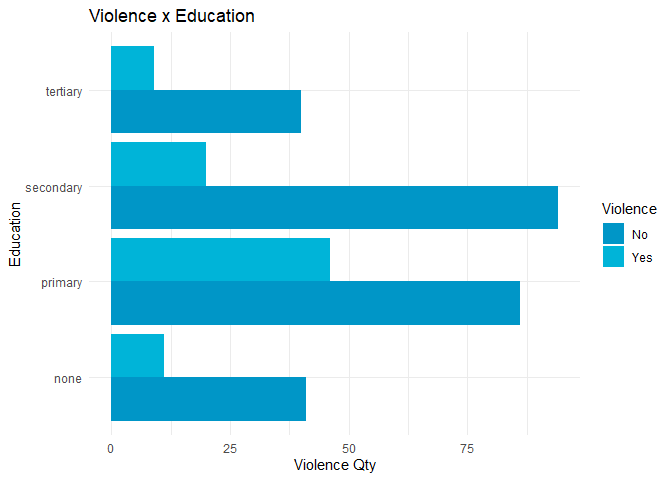
\includegraphics{Violence-On-Women_files/figure-latex/educationxviolence-1.pdf}

\hypertarget{marital-status-and-employment-for-violence-cases}{%
\subsubsection{Marital Status and Employment for Violence
cases}\label{marital-status-and-employment-for-violence-cases}}

\begin{Shaded}
\begin{Highlighting}[]
\CommentTok{\# Marital Status and Employment for Violence cases}
\NormalTok{violence\_plots }\OtherTok{\textless{}{-}}\NormalTok{ df }\SpecialCharTok{\%\textgreater{}\%}
  \FunctionTok{filter}\NormalTok{(Violence }\SpecialCharTok{==} \DecValTok{1}\NormalTok{) }\SpecialCharTok{\%\textgreater{}\%}
\NormalTok{  \{}
    \FunctionTok{list}\NormalTok{(}
      \FunctionTok{ggplot}\NormalTok{(., }\FunctionTok{aes}\NormalTok{(}\AttributeTok{x =}\NormalTok{ Marital\_status)) }\SpecialCharTok{+}
        \FunctionTok{geom\_bar}\NormalTok{(}\AttributeTok{fill =}\NormalTok{ palette[}\DecValTok{1}\NormalTok{]) }\SpecialCharTok{+}
        \FunctionTok{theme\_minimal}\NormalTok{() }\SpecialCharTok{+}
        \FunctionTok{labs}\NormalTok{(}\AttributeTok{y =} \StringTok{""}\NormalTok{),}
      
      \FunctionTok{ggplot}\NormalTok{(., }\FunctionTok{aes}\NormalTok{(}\AttributeTok{x =}\NormalTok{ Employment)) }\SpecialCharTok{+}
        \FunctionTok{geom\_bar}\NormalTok{(}\AttributeTok{fill =}\NormalTok{ palette[}\DecValTok{1}\NormalTok{]) }\SpecialCharTok{+}
        \FunctionTok{theme\_minimal}\NormalTok{() }\SpecialCharTok{+}
        \FunctionTok{labs}\NormalTok{(}\AttributeTok{y =} \StringTok{""}\NormalTok{)}
\NormalTok{    )}
\NormalTok{  \}}

\FunctionTok{grid.arrange}\NormalTok{(}\AttributeTok{grobs =}\NormalTok{ violence\_plots, }\AttributeTok{ncol =} \DecValTok{2}\NormalTok{)}
\end{Highlighting}
\end{Shaded}

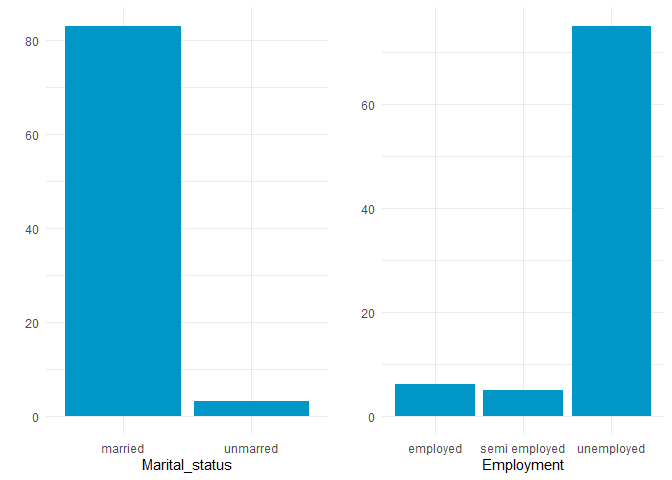
\includegraphics{Violence-On-Women_files/figure-latex/maritalstatus_employment-1.pdf}

\hypertarget{relationships-of-education-age-marital-status-and-income-with-one-another}{%
\subsubsection{Relationships of Education, Age, Marital Status, and
Income with one
another}\label{relationships-of-education-age-marital-status-and-income-with-one-another}}

\begin{Shaded}
\begin{Highlighting}[]
\CommentTok{\# Education x Age, Marital Status x Age, Education x Income}
\NormalTok{p7 }\OtherTok{\textless{}{-}} \FunctionTok{ggplot}\NormalTok{(df, }\FunctionTok{aes}\NormalTok{(}\AttributeTok{x =}\NormalTok{ Education, }\AttributeTok{y =}\NormalTok{ Age)) }\SpecialCharTok{+}
  \FunctionTok{geom\_jitter}\NormalTok{(}\AttributeTok{width =} \FloatTok{0.2}\NormalTok{) }\SpecialCharTok{+}
  \FunctionTok{theme\_minimal}\NormalTok{()}

\NormalTok{p8 }\OtherTok{\textless{}{-}} \FunctionTok{ggplot}\NormalTok{(df, }\FunctionTok{aes}\NormalTok{(}\AttributeTok{x =}\NormalTok{ Marital\_status, }\AttributeTok{y =}\NormalTok{ Age)) }\SpecialCharTok{+}
  \FunctionTok{geom\_jitter}\NormalTok{(}\AttributeTok{width =} \FloatTok{0.2}\NormalTok{) }\SpecialCharTok{+}
  \FunctionTok{theme\_minimal}\NormalTok{()}

\NormalTok{p9 }\OtherTok{\textless{}{-}} \FunctionTok{ggplot}\NormalTok{(df, }\FunctionTok{aes}\NormalTok{(}\AttributeTok{x =}\NormalTok{ Education, }\AttributeTok{y =}\NormalTok{ Income)) }\SpecialCharTok{+}
  \FunctionTok{geom\_point}\NormalTok{() }\SpecialCharTok{+}
  \FunctionTok{theme\_minimal}\NormalTok{()}

\FunctionTok{grid.arrange}\NormalTok{(p7, p8, p9, }\AttributeTok{ncol =} \DecValTok{3}\NormalTok{)}
\end{Highlighting}
\end{Shaded}

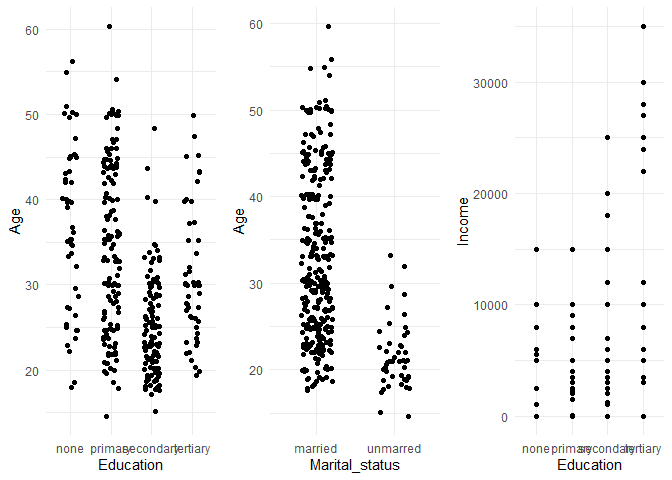
\includegraphics{Violence-On-Women_files/figure-latex/jitter_pointplots-1.pdf}

\hypertarget{average-income-per-education-level}{%
\subsubsection{Average Income per Education
Level}\label{average-income-per-education-level}}

\begin{Shaded}
\begin{Highlighting}[]
\CommentTok{\# Average income per Education Level}
\NormalTok{average\_income\_per\_education }\OtherTok{\textless{}{-}}\NormalTok{ df }\SpecialCharTok{\%\textgreater{}\%}
  \FunctionTok{group\_by}\NormalTok{(Education) }\SpecialCharTok{\%\textgreater{}\%}
  \FunctionTok{summarise}\NormalTok{(}\AttributeTok{Income =} \FunctionTok{round}\NormalTok{(}\FunctionTok{mean}\NormalTok{(Income), }\DecValTok{2}\NormalTok{)) }\SpecialCharTok{\%\textgreater{}\%}
  \FunctionTok{arrange}\NormalTok{(Income)}

\FunctionTok{print}\NormalTok{(average\_income\_per\_education)}
\end{Highlighting}
\end{Shaded}

\begin{verbatim}
## # A tibble: 4 x 2
##   Education Income
##   <chr>      <dbl>
## 1 primary     736.
## 2 none       1221.
## 3 secondary  1458.
## 4 tertiary   8276.
\end{verbatim}

\begin{Shaded}
\begin{Highlighting}[]
\FunctionTok{ggplot}\NormalTok{(average\_income\_per\_education, }\FunctionTok{aes}\NormalTok{(}\AttributeTok{x =}\NormalTok{ Education, }\AttributeTok{y =}\NormalTok{ Income, }\AttributeTok{fill =}\NormalTok{ Education)) }\SpecialCharTok{+}
  \FunctionTok{geom\_bar}\NormalTok{(}\AttributeTok{stat =} \StringTok{"identity"}\NormalTok{) }\SpecialCharTok{+}
  \FunctionTok{scale\_fill\_manual}\NormalTok{(}\AttributeTok{values =}\NormalTok{ palette) }\SpecialCharTok{+}
  \FunctionTok{theme\_minimal}\NormalTok{() }\SpecialCharTok{+}
  \FunctionTok{theme}\NormalTok{(}\AttributeTok{legend.position =} \StringTok{"none"}\NormalTok{)}
\end{Highlighting}
\end{Shaded}

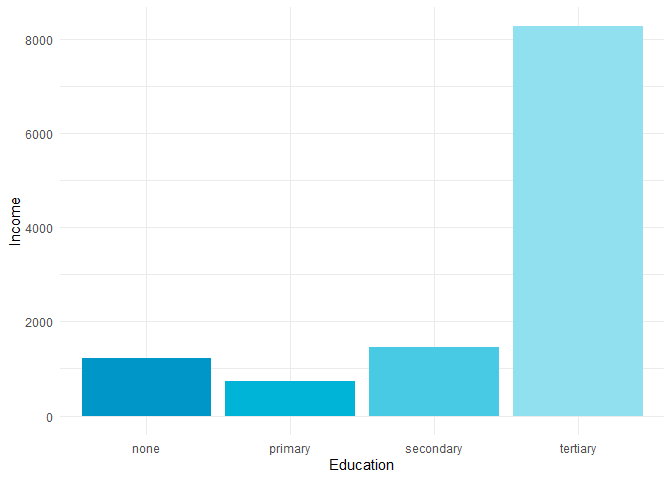
\includegraphics{Violence-On-Women_files/figure-latex/avgincome-1.pdf}

\hypertarget{binarizing-the-dataset-and-creating-dummy-variables-for-categorical-features}{%
\subsubsection{Binarizing the dataset and creating dummy variables for
categorical
features}\label{binarizing-the-dataset-and-creating-dummy-variables-for-categorical-features}}

\begin{Shaded}
\begin{Highlighting}[]
\CommentTok{\# Binarizing the dataset}
\NormalTok{binary\_features }\OtherTok{\textless{}{-}}\NormalTok{ df }\SpecialCharTok{\%\textgreater{}\%} \FunctionTok{select}\NormalTok{(Age, Income, Violence)}

\CommentTok{\# Creating dummy variables for the categorical features}
\CommentTok{\# Excluding the already binarized columns}
\NormalTok{dummie\_features }\OtherTok{\textless{}{-}}\NormalTok{ df }\SpecialCharTok{\%\textgreater{}\%} 
  \FunctionTok{select}\NormalTok{(}\SpecialCharTok{{-}}\NormalTok{Age, }\SpecialCharTok{{-}}\NormalTok{Income, }\SpecialCharTok{{-}}\NormalTok{Violence, }\SpecialCharTok{{-}}\NormalTok{marital\_binary, }\SpecialCharTok{{-}}\NormalTok{education\_binary, }\SpecialCharTok{{-}}\NormalTok{employment\_binary) }\SpecialCharTok{\%\textgreater{}\%}
  \FunctionTok{mutate}\NormalTok{(}\FunctionTok{across}\NormalTok{(}\FunctionTok{everything}\NormalTok{(), }\SpecialCharTok{\textasciitilde{}} \FunctionTok{ifelse}\NormalTok{(. }\SpecialCharTok{==} \ConstantTok{TRUE}\NormalTok{, }\DecValTok{1}\NormalTok{, }\DecValTok{0}\NormalTok{)))  }\CommentTok{\# Transform TRUE/FALSE into 1/0}

\CommentTok{\# Combining binary features with dummy features}
\NormalTok{df\_ml }\OtherTok{\textless{}{-}} \FunctionTok{cbind}\NormalTok{(binary\_features, dummie\_features)}

\CommentTok{\# Plot original dataset Violence distribution}
\NormalTok{p1 }\OtherTok{\textless{}{-}} \FunctionTok{ggplot}\NormalTok{(df\_ml, }\FunctionTok{aes}\NormalTok{(}\AttributeTok{x =} \FunctionTok{as.factor}\NormalTok{(Violence))) }\SpecialCharTok{+}
  \FunctionTok{geom\_bar}\NormalTok{(}\AttributeTok{fill =}\NormalTok{ palette[}\DecValTok{1}\NormalTok{]) }\SpecialCharTok{+}
  \FunctionTok{labs}\NormalTok{(}\AttributeTok{title =} \StringTok{"Violence Distribution in Original Data"}\NormalTok{, }\AttributeTok{x =} \StringTok{"Violence"}\NormalTok{) }\SpecialCharTok{+}
  \FunctionTok{theme\_minimal}\NormalTok{()}
\end{Highlighting}
\end{Shaded}

\hypertarget{data-resampling}{%
\subsection{Data Resampling}\label{data-resampling}}

To address class imbalance in the violence variable, the SMOTE
(Synthetic Minority Over-sampling Technique) technique is used. This
resampling method balances the dataset by generating synthetic instances
of the minority class (violence cases).

\begin{Shaded}
\begin{Highlighting}[]
\CommentTok{\# Re{-}sampling the dataset using SMOTE}
\FunctionTok{set.seed}\NormalTok{(}\DecValTok{123}\NormalTok{)  }\CommentTok{\# Set seed for reproducibility}
\FunctionTok{table}\NormalTok{(df\_ml}\SpecialCharTok{$}\NormalTok{Violence)}
\end{Highlighting}
\end{Shaded}

\begin{verbatim}
## 
##   0   1 
## 261  86
\end{verbatim}

\begin{Shaded}
\begin{Highlighting}[]
\CommentTok{\# Set N to be larger than the total number of rows in the dataset}
\NormalTok{total\_samples }\OtherTok{\textless{}{-}} \FunctionTok{nrow}\NormalTok{(df\_ml)}
\NormalTok{N\_target }\OtherTok{\textless{}{-}} \DecValTok{2} \SpecialCharTok{*}\NormalTok{ total\_samples  }\CommentTok{\# Set to twice the total number of rows to ensure oversampling}

\CommentTok{\# Apply SMOTE using the larger N value}
\NormalTok{smote\_data }\OtherTok{\textless{}{-}} \FunctionTok{ovun.sample}\NormalTok{(Violence }\SpecialCharTok{\textasciitilde{}}\NormalTok{ ., }\AttributeTok{data =}\NormalTok{ df\_ml, }\AttributeTok{method =} \StringTok{"over"}\NormalTok{, }\AttributeTok{N =}\NormalTok{ N\_target)}\SpecialCharTok{$}\NormalTok{data}

\CommentTok{\# Plot resampled dataset Violence distribution}
\NormalTok{p2 }\OtherTok{\textless{}{-}} \FunctionTok{ggplot}\NormalTok{(smote\_data, }\FunctionTok{aes}\NormalTok{(}\AttributeTok{x =} \FunctionTok{as.factor}\NormalTok{(Violence))) }\SpecialCharTok{+}
  \FunctionTok{geom\_bar}\NormalTok{(}\AttributeTok{fill =}\NormalTok{ palette[}\DecValTok{1}\NormalTok{]) }\SpecialCharTok{+}
  \FunctionTok{labs}\NormalTok{(}\AttributeTok{title =} \StringTok{"Violence Distribution after SMOTE"}\NormalTok{, }\AttributeTok{x =} \StringTok{"Violence"}\NormalTok{) }\SpecialCharTok{+}
  \FunctionTok{theme\_minimal}\NormalTok{()}

\CommentTok{\# Arrange both plots side by side}
\FunctionTok{grid.arrange}\NormalTok{(p1, p2, }\AttributeTok{ncol =} \DecValTok{2}\NormalTok{)}
\end{Highlighting}
\end{Shaded}

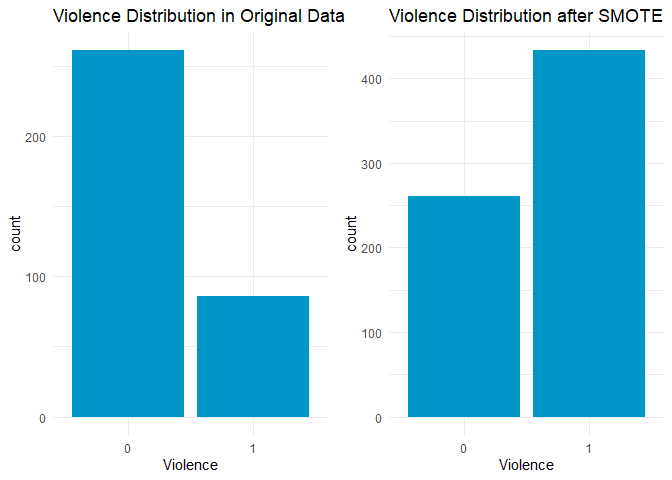
\includegraphics{Violence-On-Women_files/figure-latex/data_resampling-1.pdf}

\begin{Shaded}
\begin{Highlighting}[]
\CommentTok{\# Randomly shuffle the resampled dataset}
\NormalTok{df\_ml\_sample }\OtherTok{\textless{}{-}}\NormalTok{ smote\_data[}\FunctionTok{sample}\NormalTok{(}\FunctionTok{nrow}\NormalTok{(smote\_data)), ]}

\NormalTok{SEED }\OtherTok{\textless{}{-}} \DecValTok{158020}
\FunctionTok{set.seed}\NormalTok{(SEED)}

\CommentTok{\# Prepare the dataset: Exclude the \textquotesingle{}Violence\textquotesingle{} column from features (X) and define the target (y)}
\NormalTok{x }\OtherTok{\textless{}{-}}\NormalTok{ df\_ml\_sample }\SpecialCharTok{\%\textgreater{}\%} \FunctionTok{select}\NormalTok{(}\SpecialCharTok{{-}}\NormalTok{Violence)}
\NormalTok{y }\OtherTok{\textless{}{-}}\NormalTok{ df\_ml\_sample}\SpecialCharTok{$}\NormalTok{Violence}

\CommentTok{\# Normalize the features using the preProcess function from the caret package}
\NormalTok{norm }\OtherTok{\textless{}{-}} \FunctionTok{preProcess}\NormalTok{(x, }\AttributeTok{method =} \FunctionTok{c}\NormalTok{(}\StringTok{"center"}\NormalTok{, }\StringTok{"scale"}\NormalTok{))}
\NormalTok{x\_norm }\OtherTok{\textless{}{-}} \FunctionTok{predict}\NormalTok{(norm, x)}
\end{Highlighting}
\end{Shaded}

\hypertarget{model-training-and-evaluation}{%
\subsection{Model Training and
Evaluation}\label{model-training-and-evaluation}}

\hypertarget{baseline-and-predictive-models}{%
\subsubsection{Baseline and Predictive
Models}\label{baseline-and-predictive-models}}

\begin{Shaded}
\begin{Highlighting}[]
\CommentTok{\# Split the data into training and testing sets}
\FunctionTok{set.seed}\NormalTok{(}\DecValTok{123}\NormalTok{)}
\NormalTok{trainIndex }\OtherTok{\textless{}{-}} \FunctionTok{createDataPartition}\NormalTok{(y, }\AttributeTok{p =} \FloatTok{0.7}\NormalTok{, }\AttributeTok{list =} \ConstantTok{FALSE}\NormalTok{)}
\NormalTok{train\_x }\OtherTok{\textless{}{-}}\NormalTok{ x\_norm[trainIndex, ]}
\NormalTok{test\_x }\OtherTok{\textless{}{-}}\NormalTok{ x\_norm[}\SpecialCharTok{{-}}\NormalTok{trainIndex, ]}
\NormalTok{train\_y }\OtherTok{\textless{}{-}}\NormalTok{ y[trainIndex]}
\NormalTok{test\_y }\OtherTok{\textless{}{-}}\NormalTok{ y[}\SpecialCharTok{{-}}\NormalTok{trainIndex]}

\CommentTok{\# Function to run model scores}
\NormalTok{model }\OtherTok{\textless{}{-}} \ControlFlowTok{function}\NormalTok{(model, test\_x, test\_y) \{}
\NormalTok{  predictions }\OtherTok{\textless{}{-}} \FunctionTok{predict}\NormalTok{(model, }\AttributeTok{newdata =}\NormalTok{ test\_x)}
\NormalTok{  accuracy }\OtherTok{\textless{}{-}} \FunctionTok{mean}\NormalTok{(predictions }\SpecialCharTok{==}\NormalTok{ test\_y) }\SpecialCharTok{*} \DecValTok{100}
\NormalTok{  conf\_matrix }\OtherTok{\textless{}{-}} \FunctionTok{confusionMatrix}\NormalTok{(predictions, }\FunctionTok{as.factor}\NormalTok{(test\_y))}
  
  \FunctionTok{print}\NormalTok{(conf\_matrix)}
  \FunctionTok{print}\NormalTok{(}\FunctionTok{sprintf}\NormalTok{(}\StringTok{"Accuracy: \%.2f\%\%"}\NormalTok{, accuracy))}
\NormalTok{\}}
\end{Highlighting}
\end{Shaded}

Baseline Random Forest: Establishes a benchmark for accuracy against
which other models are compared.

\begin{Shaded}
\begin{Highlighting}[]
\CommentTok{\# Dummy Classifier {-} Baseline}
\NormalTok{dummy\_model }\OtherTok{\textless{}{-}} \FunctionTok{train}\NormalTok{(train\_x, }\FunctionTok{as.factor}\NormalTok{(train\_y), }\AttributeTok{method =} \StringTok{"rf"}\NormalTok{, }\AttributeTok{trControl =} \FunctionTok{trainControl}\NormalTok{(}\AttributeTok{method =} \StringTok{"cv"}\NormalTok{, }\AttributeTok{number =} \DecValTok{5}\NormalTok{))}
\FunctionTok{model}\NormalTok{(dummy\_model, test\_x, test\_y)}
\end{Highlighting}
\end{Shaded}

\begin{verbatim}
## Confusion Matrix and Statistics
## 
##           Reference
## Prediction   0   1
##          0  32  17
##          1  49 110
##                                           
##                Accuracy : 0.6827          
##                  95% CI : (0.6148, 0.7453)
##     No Information Rate : 0.6106          
##     P-Value [Acc > NIR] : 0.0186548       
##                                           
##                   Kappa : 0.2813          
##                                           
##  Mcnemar's Test P-Value : 0.0001357       
##                                           
##             Sensitivity : 0.3951          
##             Specificity : 0.8661          
##          Pos Pred Value : 0.6531          
##          Neg Pred Value : 0.6918          
##              Prevalence : 0.3894          
##          Detection Rate : 0.1538          
##    Detection Prevalence : 0.2356          
##       Balanced Accuracy : 0.6306          
##                                           
##        'Positive' Class : 0               
##                                           
## [1] "Accuracy: 68.27%"
\end{verbatim}

Naive Bayes Classifier: A simple probabilistic classifier based on
Bayes' theorem.

\begin{Shaded}
\begin{Highlighting}[]
\CommentTok{\# Naive Bayes Classifier}
\NormalTok{nb\_model }\OtherTok{\textless{}{-}} \FunctionTok{naiveBayes}\NormalTok{(}\FunctionTok{as.factor}\NormalTok{(train\_y) }\SpecialCharTok{\textasciitilde{}}\NormalTok{ ., }\AttributeTok{data =}\NormalTok{ train\_x)}
\FunctionTok{model}\NormalTok{(nb\_model, test\_x, test\_y)}
\end{Highlighting}
\end{Shaded}

\begin{verbatim}
## Confusion Matrix and Statistics
## 
##           Reference
## Prediction   0   1
##          0   7   2
##          1  74 125
##                                           
##                Accuracy : 0.6346          
##                  95% CI : (0.5652, 0.7001)
##     No Information Rate : 0.6106          
##     P-Value [Acc > NIR] : 0.2622          
##                                           
##                   Kappa : 0.0842          
##                                           
##  Mcnemar's Test P-Value : 3.816e-16       
##                                           
##             Sensitivity : 0.08642         
##             Specificity : 0.98425         
##          Pos Pred Value : 0.77778         
##          Neg Pred Value : 0.62814         
##              Prevalence : 0.38942         
##          Detection Rate : 0.03365         
##    Detection Prevalence : 0.04327         
##       Balanced Accuracy : 0.53534         
##                                           
##        'Positive' Class : 0               
##                                           
## [1] "Accuracy: 63.46%"
\end{verbatim}

Decision Tree: Provides interpretable results to identify key features
influencing violence.

\begin{Shaded}
\begin{Highlighting}[]
\CommentTok{\# Decision Tree Classifier}
\NormalTok{tree\_model }\OtherTok{\textless{}{-}} \FunctionTok{rpart}\NormalTok{(}\FunctionTok{as.factor}\NormalTok{(train\_y) }\SpecialCharTok{\textasciitilde{}}\NormalTok{ ., }\AttributeTok{data =}\NormalTok{ train\_x, }\AttributeTok{method =} \StringTok{"class"}\NormalTok{, }\AttributeTok{control =} \FunctionTok{rpart.control}\NormalTok{(}\AttributeTok{maxdepth =} \DecValTok{2}\NormalTok{))}

\CommentTok{\# Updated model function to ensure class predictions for decision trees}
\NormalTok{model }\OtherTok{\textless{}{-}} \ControlFlowTok{function}\NormalTok{(model, test\_x, test\_y) \{}
  \ControlFlowTok{if}\NormalTok{ (}\StringTok{"rpart"} \SpecialCharTok{\%in\%} \FunctionTok{class}\NormalTok{(model)) \{}
    \CommentTok{\# For rpart models, get class predictions directly}
\NormalTok{    predictions }\OtherTok{\textless{}{-}} \FunctionTok{predict}\NormalTok{(model, }\AttributeTok{newdata =}\NormalTok{ test\_x, }\AttributeTok{type =} \StringTok{"class"}\NormalTok{)}
\NormalTok{  \} }\ControlFlowTok{else}\NormalTok{ \{}
    \CommentTok{\# For other models, assume normal predict works fine}
\NormalTok{    predictions }\OtherTok{\textless{}{-}} \FunctionTok{predict}\NormalTok{(model, }\AttributeTok{newdata =}\NormalTok{ test\_x)}
\NormalTok{  \}}
  
\NormalTok{  accuracy }\OtherTok{\textless{}{-}} \FunctionTok{mean}\NormalTok{(predictions }\SpecialCharTok{==}\NormalTok{ test\_y) }\SpecialCharTok{*} \DecValTok{100}
\NormalTok{  conf\_matrix }\OtherTok{\textless{}{-}} \FunctionTok{confusionMatrix}\NormalTok{(predictions, }\FunctionTok{as.factor}\NormalTok{(test\_y))}
  
  \FunctionTok{print}\NormalTok{(conf\_matrix)}
  \FunctionTok{print}\NormalTok{(}\FunctionTok{sprintf}\NormalTok{(}\StringTok{"Accuracy: \%.2f\%\%"}\NormalTok{, accuracy))}
\NormalTok{\}}

\CommentTok{\# Run the model evaluation again for Decision Tree}
\FunctionTok{model}\NormalTok{(tree\_model, test\_x, test\_y)}
\end{Highlighting}
\end{Shaded}

\begin{verbatim}
## Confusion Matrix and Statistics
## 
##           Reference
## Prediction   0   1
##          0  13  21
##          1  68 106
##                                           
##                Accuracy : 0.5721          
##                  95% CI : (0.5018, 0.6403)
##     No Information Rate : 0.6106          
##     P-Value [Acc > NIR] : 0.8862          
##                                           
##                   Kappa : -0.0054         
##                                           
##  Mcnemar's Test P-Value : 1.083e-06       
##                                           
##             Sensitivity : 0.1605          
##             Specificity : 0.8346          
##          Pos Pred Value : 0.3824          
##          Neg Pred Value : 0.6092          
##              Prevalence : 0.3894          
##          Detection Rate : 0.0625          
##    Detection Prevalence : 0.1635          
##       Balanced Accuracy : 0.4976          
##                                           
##        'Positive' Class : 0               
##                                           
## [1] "Accuracy: 57.21%"
\end{verbatim}

K-Nearest Neighbors (KNN): Applied with both Euclidean and Hamming
distances.

\begin{Shaded}
\begin{Highlighting}[]
\CommentTok{\# K{-}Nearest Neighbors (KNN)}
\CommentTok{\# With Euclidean distance}
\NormalTok{knn\_model\_euclidean }\OtherTok{\textless{}{-}} \FunctionTok{knn}\NormalTok{(}\AttributeTok{train =}\NormalTok{ train\_x, }\AttributeTok{test =}\NormalTok{ test\_x, }\AttributeTok{cl =}\NormalTok{ train\_y, }\AttributeTok{k =} \DecValTok{5}\NormalTok{)}
\FunctionTok{confusionMatrix}\NormalTok{(knn\_model\_euclidean, }\FunctionTok{as.factor}\NormalTok{(test\_y))}
\end{Highlighting}
\end{Shaded}

\begin{verbatim}
## Confusion Matrix and Statistics
## 
##           Reference
## Prediction   0   1
##          0  17  20
##          1  64 107
##                                           
##                Accuracy : 0.5962          
##                  95% CI : (0.5261, 0.6634)
##     No Information Rate : 0.6106          
##     P-Value [Acc > NIR] : 0.692           
##                                           
##                   Kappa : 0.0581          
##                                           
##  Mcnemar's Test P-Value : 2.71e-06        
##                                           
##             Sensitivity : 0.20988         
##             Specificity : 0.84252         
##          Pos Pred Value : 0.45946         
##          Neg Pred Value : 0.62573         
##              Prevalence : 0.38942         
##          Detection Rate : 0.08173         
##    Detection Prevalence : 0.17788         
##       Balanced Accuracy : 0.52620         
##                                           
##        'Positive' Class : 0               
## 
\end{verbatim}

\begin{Shaded}
\begin{Highlighting}[]
\CommentTok{\# With Hamming distance (more suitable for binary data)}
\NormalTok{knn\_model\_hamming }\OtherTok{\textless{}{-}} \FunctionTok{knn}\NormalTok{(}\AttributeTok{train =}\NormalTok{ train\_x, }\AttributeTok{test =}\NormalTok{ test\_x, }\AttributeTok{cl =}\NormalTok{ train\_y, }\AttributeTok{k =} \DecValTok{4}\NormalTok{)}
\FunctionTok{confusionMatrix}\NormalTok{(knn\_model\_hamming, }\FunctionTok{as.factor}\NormalTok{(test\_y))}
\end{Highlighting}
\end{Shaded}

\begin{verbatim}
## Confusion Matrix and Statistics
## 
##           Reference
## Prediction   0   1
##          0  19  20
##          1  62 107
##                                           
##                Accuracy : 0.6058          
##                  95% CI : (0.5358, 0.6726)
##     No Information Rate : 0.6106          
##     P-Value [Acc > NIR] : 0.5864          
##                                           
##                   Kappa : 0.0851          
##                                           
##  Mcnemar's Test P-Value : 5.963e-06       
##                                           
##             Sensitivity : 0.23457         
##             Specificity : 0.84252         
##          Pos Pred Value : 0.48718         
##          Neg Pred Value : 0.63314         
##              Prevalence : 0.38942         
##          Detection Rate : 0.09135         
##    Detection Prevalence : 0.18750         
##       Balanced Accuracy : 0.53854         
##                                           
##        'Positive' Class : 0               
## 
\end{verbatim}

Random Forest: Offers higher accuracy by averaging multiple decision
trees.

\begin{Shaded}
\begin{Highlighting}[]
\CommentTok{\# Random Forest Classifier}
\NormalTok{rf\_model }\OtherTok{\textless{}{-}} \FunctionTok{randomForest}\NormalTok{(}\FunctionTok{as.factor}\NormalTok{(train\_y) }\SpecialCharTok{\textasciitilde{}}\NormalTok{ ., }\AttributeTok{data =}\NormalTok{ train\_x, }\AttributeTok{ntree =} \DecValTok{100}\NormalTok{)}
\FunctionTok{model}\NormalTok{(rf\_model, test\_x, test\_y)}
\end{Highlighting}
\end{Shaded}

\begin{verbatim}
## Confusion Matrix and Statistics
## 
##           Reference
## Prediction   0   1
##          0  11  10
##          1  70 117
##                                           
##                Accuracy : 0.6154          
##                  95% CI : (0.5456, 0.6818)
##     No Information Rate : 0.6106          
##     P-Value [Acc > NIR] : 0.4738          
##                                           
##                   Kappa : 0.0659          
##                                           
##  Mcnemar's Test P-Value : 4.213e-11       
##                                           
##             Sensitivity : 0.13580         
##             Specificity : 0.92126         
##          Pos Pred Value : 0.52381         
##          Neg Pred Value : 0.62567         
##              Prevalence : 0.38942         
##          Detection Rate : 0.05288         
##    Detection Prevalence : 0.10096         
##       Balanced Accuracy : 0.52853         
##                                           
##        'Positive' Class : 0               
##                                           
## [1] "Accuracy: 61.54%"
\end{verbatim}

\begin{Shaded}
\begin{Highlighting}[]
\CommentTok{\# Define a function to print results}
\NormalTok{print\_results }\OtherTok{\textless{}{-}} \ControlFlowTok{function}\NormalTok{(results) \{}
\NormalTok{  mean\_acc }\OtherTok{\textless{}{-}} \FunctionTok{mean}\NormalTok{(results}\SpecialCharTok{$}\NormalTok{results}\SpecialCharTok{$}\NormalTok{Accuracy)}
\NormalTok{  std\_acc }\OtherTok{\textless{}{-}} \FunctionTok{sd}\NormalTok{(results}\SpecialCharTok{$}\NormalTok{results}\SpecialCharTok{$}\NormalTok{Accuracy)}
  \FunctionTok{cat}\NormalTok{(}\FunctionTok{sprintf}\NormalTok{(}\StringTok{"Average Accuracy: \%.2f\%\%}\SpecialCharTok{\textbackslash{}n}\StringTok{"}\NormalTok{, mean\_acc }\SpecialCharTok{*} \DecValTok{100}\NormalTok{))}
  \FunctionTok{cat}\NormalTok{(}\FunctionTok{sprintf}\NormalTok{(}\StringTok{"Accuracy interval: [\%.2f, \%.2f]\%\%}\SpecialCharTok{\textbackslash{}n}\StringTok{"}\NormalTok{, (mean\_acc }\SpecialCharTok{{-}} \DecValTok{2} \SpecialCharTok{*}\NormalTok{ std\_acc) }\SpecialCharTok{*} \DecValTok{100}\NormalTok{, (mean\_acc }\SpecialCharTok{+} \DecValTok{2} \SpecialCharTok{*}\NormalTok{ std\_acc) }\SpecialCharTok{*} \DecValTok{100}\NormalTok{))}
\NormalTok{\}}
\end{Highlighting}
\end{Shaded}

\hypertarget{model-performance-evaluation}{%
\subsubsection{Model Performance
Evaluation}\label{model-performance-evaluation}}

Confusion Matrix and Accuracy: Each model's performance is evaluated
using accuracy and confusion matrix metrics to assess the classification
quality.

Cross-Validation: All models undergo cross-validation to provide robust
performance metrics and avoid overfitting.

\begin{Shaded}
\begin{Highlighting}[]
\CommentTok{\# Set random seed}
\FunctionTok{set.seed}\NormalTok{(}\DecValTok{158020}\NormalTok{)}

\CommentTok{\# Define cross{-}validation method}
\NormalTok{train\_control }\OtherTok{\textless{}{-}} \FunctionTok{trainControl}\NormalTok{(}\AttributeTok{method =} \StringTok{"cv"}\NormalTok{, }\AttributeTok{number =} \DecValTok{10}\NormalTok{)}

\CommentTok{\# Prepare the dataset (x and y are from previous steps, assuming they are ready)}
\CommentTok{\# x\_norm and y are normalized features and target (Violence) from the previous steps}

\CommentTok{\# Ensure y is named properly and combine with x\_norm}
\NormalTok{df\_combined }\OtherTok{\textless{}{-}} \FunctionTok{cbind}\NormalTok{(x\_norm, }\AttributeTok{Violence =}\NormalTok{ y)  }\CommentTok{\# Rename your target variable appropriately}

\CommentTok{\# Check column names of df\_combined to ensure there\textquotesingle{}s no mismatch}
\FunctionTok{colnames}\NormalTok{(df\_combined)}
\end{Highlighting}
\end{Shaded}

\begin{verbatim}
## [1] "Age"            "Income"         "Education"      "Employment"    
## [5] "Marital_status" "Violence"
\end{verbatim}

\begin{Shaded}
\begin{Highlighting}[]
\CommentTok{\# Decision Tree Classifier with cross{-}validation}
\NormalTok{tree\_model }\OtherTok{\textless{}{-}} \FunctionTok{train}\NormalTok{(}\FunctionTok{as.factor}\NormalTok{(Violence) }\SpecialCharTok{\textasciitilde{}}\NormalTok{ ., }\AttributeTok{data =}\NormalTok{ df\_combined, }
                    \AttributeTok{method =} \StringTok{"rpart"}\NormalTok{, }
                    \AttributeTok{trControl =}\NormalTok{ train\_control, }
                    \AttributeTok{tuneGrid =} \FunctionTok{expand.grid}\NormalTok{(}\AttributeTok{cp =} \FloatTok{0.01}\NormalTok{),  }\CommentTok{\# Cross{-}validation on complexity parameter}
                    \AttributeTok{control =} \FunctionTok{rpart.control}\NormalTok{(}\AttributeTok{maxdepth =} \DecValTok{2}\NormalTok{))}

\CommentTok{\# Check the results}
\NormalTok{tree\_model}
\end{Highlighting}
\end{Shaded}

\begin{verbatim}
## CART 
## 
## 694 samples
##   5 predictor
##   2 classes: '0', '1' 
## 
## No pre-processing
## Resampling: Cross-Validated (10 fold) 
## Summary of sample sizes: 625, 625, 625, 624, 625, 625, ... 
## Resampling results:
## 
##   Accuracy   Kappa     
##   0.6310766  0.07216199
## 
## Tuning parameter 'cp' was held constant at a value of 0.01
\end{verbatim}

\begin{Shaded}
\begin{Highlighting}[]
\CommentTok{\# Print cross{-}validation results for Decision Tree}
\FunctionTok{print\_results}\NormalTok{(tree\_model)}
\end{Highlighting}
\end{Shaded}

\begin{verbatim}
## Average Accuracy: 63.11%
## Accuracy interval: [NA, NA]%
\end{verbatim}

\begin{Shaded}
\begin{Highlighting}[]
\CommentTok{\# K{-}Nearest Neighbors with cross{-}validation}
\NormalTok{knn\_model }\OtherTok{\textless{}{-}} \FunctionTok{train}\NormalTok{(}\FunctionTok{as.factor}\NormalTok{(Violence) }\SpecialCharTok{\textasciitilde{}}\NormalTok{ ., }\AttributeTok{data =}\NormalTok{ df\_combined, }
                   \AttributeTok{method =} \StringTok{"knn"}\NormalTok{, }
                   \AttributeTok{metric =} \StringTok{"Accuracy"}\NormalTok{, }
                   \AttributeTok{tuneGrid =} \FunctionTok{expand.grid}\NormalTok{(}\AttributeTok{k =} \DecValTok{3}\NormalTok{),  }\CommentTok{\# 3 neighbors}
                   \AttributeTok{trControl =}\NormalTok{ train\_control)}

\CommentTok{\# Print cross{-}validation results for KNN}
\FunctionTok{print\_results}\NormalTok{(knn\_model)}
\end{Highlighting}
\end{Shaded}

\begin{verbatim}
## Average Accuracy: 69.62%
## Accuracy interval: [NA, NA]%
\end{verbatim}

\begin{Shaded}
\begin{Highlighting}[]
\CommentTok{\# Random Forest with cross{-}validation}
\NormalTok{rf\_model }\OtherTok{\textless{}{-}} \FunctionTok{train}\NormalTok{(}\FunctionTok{as.factor}\NormalTok{(Violence) }\SpecialCharTok{\textasciitilde{}}\NormalTok{ ., }\AttributeTok{data =}\NormalTok{ df\_combined, }
                  \AttributeTok{method =} \StringTok{"rf"}\NormalTok{, }
                  \AttributeTok{trControl =}\NormalTok{ train\_control, }
                  \AttributeTok{tuneGrid =} \FunctionTok{expand.grid}\NormalTok{(}\AttributeTok{mtry =} \DecValTok{3}\NormalTok{))  }\CommentTok{\# mtry can be adjusted or optimized}

\CommentTok{\# Print cross{-}validation results for Random Forest}
\FunctionTok{print\_results}\NormalTok{(rf\_model)}
\end{Highlighting}
\end{Shaded}

\begin{verbatim}
## Average Accuracy: 68.01%
## Accuracy interval: [NA, NA]%
\end{verbatim}

\hypertarget{hyperparameter-tuning}{%
\subsubsection{Hyperparameter Tuning}\label{hyperparameter-tuning}}

Grid Search for KNN and Random Forest: An optimal number of neighbors
(k) for KNN and best `mtry' values for Random Forest are identified
using grid search, maximizing accuracy.

\begin{Shaded}
\begin{Highlighting}[]
\CommentTok{\# Grid Search for KNN (search for optimal \textquotesingle{}k\textquotesingle{})}
\NormalTok{knn\_grid }\OtherTok{\textless{}{-}} \FunctionTok{expand.grid}\NormalTok{(}\AttributeTok{k =} \DecValTok{1}\SpecialCharTok{:}\DecValTok{31}\NormalTok{)  }\CommentTok{\# Searching k from 1 to 31}

\NormalTok{knn\_grid\_search }\OtherTok{\textless{}{-}} \FunctionTok{train}\NormalTok{(}\FunctionTok{as.factor}\NormalTok{(Violence) }\SpecialCharTok{\textasciitilde{}}\NormalTok{ ., }\AttributeTok{data =}\NormalTok{ df\_combined, }
                         \AttributeTok{method =} \StringTok{"knn"}\NormalTok{, }
                         \AttributeTok{trControl =} \FunctionTok{trainControl}\NormalTok{(}\AttributeTok{method =} \StringTok{"cv"}\NormalTok{, }\AttributeTok{number =} \DecValTok{10}\NormalTok{), }
                         \AttributeTok{tuneGrid =}\NormalTok{ knn\_grid)}

\CommentTok{\# Make predictions using the best model from Grid Search}
\NormalTok{knn\_predictions }\OtherTok{\textless{}{-}} \FunctionTok{predict}\NormalTok{(knn\_grid\_search, }\AttributeTok{newdata =}\NormalTok{ test\_x)}

\CommentTok{\# Evaluate the KNN model}
\FunctionTok{confusionMatrix}\NormalTok{(knn\_predictions, }\FunctionTok{as.factor}\NormalTok{(test\_y))}
\end{Highlighting}
\end{Shaded}

\begin{verbatim}
## Confusion Matrix and Statistics
## 
##           Reference
## Prediction   0   1
##          0  42   9
##          1  39 118
##                                           
##                Accuracy : 0.7692          
##                  95% CI : (0.7059, 0.8247)
##     No Information Rate : 0.6106          
##     P-Value [Acc > NIR] : 8.690e-07       
##                                           
##                   Kappa : 0.4798          
##                                           
##  Mcnemar's Test P-Value : 2.842e-05       
##                                           
##             Sensitivity : 0.5185          
##             Specificity : 0.9291          
##          Pos Pred Value : 0.8235          
##          Neg Pred Value : 0.7516          
##              Prevalence : 0.3894          
##          Detection Rate : 0.2019          
##    Detection Prevalence : 0.2452          
##       Balanced Accuracy : 0.7238          
##                                           
##        'Positive' Class : 0               
## 
\end{verbatim}

\begin{Shaded}
\begin{Highlighting}[]
\FunctionTok{cat}\NormalTok{(}\StringTok{"Best number of neighbors:"}\NormalTok{, knn\_grid\_search}\SpecialCharTok{$}\NormalTok{bestTune}\SpecialCharTok{$}\NormalTok{k, }\StringTok{"}\SpecialCharTok{\textbackslash{}n}\StringTok{"}\NormalTok{)}
\end{Highlighting}
\end{Shaded}

\begin{verbatim}
## Best number of neighbors: 1
\end{verbatim}

\begin{Shaded}
\begin{Highlighting}[]
\CommentTok{\# Define the tuning grid for mtry (number of predictors randomly sampled at each split)}
\NormalTok{rf\_grid }\OtherTok{\textless{}{-}} \FunctionTok{expand.grid}\NormalTok{(}\AttributeTok{mtry =} \FunctionTok{c}\NormalTok{(}\DecValTok{1}\NormalTok{, }\DecValTok{2}\NormalTok{, }\DecValTok{3}\NormalTok{, }\DecValTok{4}\NormalTok{, }\DecValTok{5}\NormalTok{))  }\CommentTok{\# Adjust values as needed}

\CommentTok{\# Perform grid search with cross{-}validation for Random Forest}
\NormalTok{rf\_grid\_search }\OtherTok{\textless{}{-}} \FunctionTok{train}\NormalTok{(}\FunctionTok{as.factor}\NormalTok{(Violence) }\SpecialCharTok{\textasciitilde{}}\NormalTok{ ., }\AttributeTok{data =}\NormalTok{ df\_combined, }
                        \AttributeTok{method =} \StringTok{"rf"}\NormalTok{, }
                        \AttributeTok{trControl =} \FunctionTok{trainControl}\NormalTok{(}\AttributeTok{method =} \StringTok{"cv"}\NormalTok{, }\AttributeTok{number =} \DecValTok{10}\NormalTok{), }
                        \AttributeTok{tuneGrid =}\NormalTok{ rf\_grid)  }\CommentTok{\# Use the proper tuneGrid with mtry}

\CommentTok{\# Check the results}
\NormalTok{rf\_grid\_search}
\end{Highlighting}
\end{Shaded}

\begin{verbatim}
## Random Forest 
## 
## 694 samples
##   5 predictor
##   2 classes: '0', '1' 
## 
## No pre-processing
## Resampling: Cross-Validated (10 fold) 
## Summary of sample sizes: 625, 625, 625, 625, 625, 624, ... 
## Resampling results across tuning parameters:
## 
##   mtry  Accuracy   Kappa     
##   1     0.6340580  0.04775053
##   2     0.6470393  0.08380190
##   3     0.6816563  0.19637691
##   4     0.7348447  0.36946612
##   5     0.7319876  0.37403343
## 
## Accuracy was used to select the optimal model using the largest value.
## The final value used for the model was mtry = 4.
\end{verbatim}

\begin{Shaded}
\begin{Highlighting}[]
\CommentTok{\# Make predictions using the best Random Forest model from Grid Search}
\NormalTok{rf\_predictions }\OtherTok{\textless{}{-}} \FunctionTok{predict}\NormalTok{(rf\_grid\_search, }\AttributeTok{newdata =}\NormalTok{ test\_x)}

\CommentTok{\# Evaluate the Random Forest model}
\FunctionTok{confusionMatrix}\NormalTok{(rf\_predictions, }\FunctionTok{as.factor}\NormalTok{(test\_y))}
\end{Highlighting}
\end{Shaded}

\begin{verbatim}
## Confusion Matrix and Statistics
## 
##           Reference
## Prediction   0   1
##          0  41   8
##          1  40 119
##                                           
##                Accuracy : 0.7692          
##                  95% CI : (0.7059, 0.8247)
##     No Information Rate : 0.6106          
##     P-Value [Acc > NIR] : 8.69e-07        
##                                           
##                   Kappa : 0.4773          
##                                           
##  Mcnemar's Test P-Value : 7.66e-06        
##                                           
##             Sensitivity : 0.5062          
##             Specificity : 0.9370          
##          Pos Pred Value : 0.8367          
##          Neg Pred Value : 0.7484          
##              Prevalence : 0.3894          
##          Detection Rate : 0.1971          
##    Detection Prevalence : 0.2356          
##       Balanced Accuracy : 0.7216          
##                                           
##        'Positive' Class : 0               
## 
\end{verbatim}

\hypertarget{results-and-discussion}{%
\subsection{Results and Discussion}\label{results-and-discussion}}

\hypertarget{comparison-of-models}{%
\subsubsection{Comparison of Models:}\label{comparison-of-models}}

Accuracy metrics reveal that Random Forest consistently provides strong
performance, followed by the Decision Tree and Naive Bayes models.

\hypertarget{interpretation-of-findings}{%
\subsubsection{Interpretation of
Findings:}\label{interpretation-of-findings}}

Education level, employment status, and age appear to correlate with the
likelihood of violence cases. Employment status and marital status are
prominent indicators in the classification of violence cases.

\hypertarget{conclusion}{%
\subsection{Conclusion}\label{conclusion}}

This analysis effectively identifies patterns associated with domestic
violence using multiple machine learning techniques. Random Forest and
Decision Tree classifiers offer high accuracy and are suitable for
interpreting feature importance. Our findings underscore the impact of
socioeconomic factors on violence prevalence, and these models can
assist in targeted interventions. Future work could expand on this
analysis by incorporating additional features and testing on larger
datasets for broader applicability.

\end{document}
